\documentclass[aspectratio=169,11pt]{beamer}

\usetheme[progressbar=frametitle]{metropolis}
\setbeamertemplate{navigation symbols}{}

\usepackage{amsmath,amssymb}
\usepackage{booktabs}
\usepackage{graphicx}
\usepackage{hyperref}
\usepackage{multimedia}
\usepackage{tikz}
\usepackage{etoolbox}

\usetikzlibrary{calc,positioning}

% Reusable research-strand triangle.
% Usage: \ResearchTriangle{mode}
%        \ResearchTriangleCorner{mode}
%   mode ∈ {off, none, all, stats-physics, stats-fp, fp-physics}
%
% Vertices (clockwise from top):
%   Statistics
%   Functional Programming
%   Physics
%
% Edges:
%   stats-physics : Statistics -- Physics              (HMC / spin-fermion)
%   stats-fp      : Statistics -- Functional Programming (FRP)
%   fp-physics    : Functional Programming -- Physics  (typed fusion)

\newcommand{\currentEdge}{off}

\newcommand{\ResearchTriangle}[1]{%
  \begin{tikzpicture}[
    baseline=(current bounding box.center),
    every node/.style={font=\sffamily},
    edge dim/.style={draw=black!28, line width=1.0pt, line cap=round},
    edge hi/.style={draw=black!88, line width=2.4pt, line cap=round},
    vtx/.style={circle, fill=black!88, draw=white, line width=1.2pt, inner sep=0pt, minimum size=2.4mm},
    lab/.style={align=center, font=\small\sffamily\bfseries, text=black!88, inner sep=1pt},
  ]
    \def\triMode{#1}
    \coordinate (S) at (90:2.35);
    \coordinate (F) at (210:2.35);
    \coordinate (P) at (330:2.35);

    \draw[edge dim] (S) -- (F);
    \draw[edge dim] (S) -- (P);
    \draw[edge dim] (F) -- (P);

    \ifstrequal{\triMode}{all}{%
      \draw[edge hi] (S) -- (F);
      \draw[edge hi] (S) -- (P);
      \draw[edge hi] (F) -- (P);
    }{}
    \ifstrequal{\triMode}{stats-fp}{%
      \draw[edge hi] (S) -- (F);
    }{}
    \ifstrequal{\triMode}{bayes-fp}{%
      \draw[edge hi] (S) -- (F);
    }{}
    \ifstrequal{\triMode}{stats-physics}{%
      \draw[edge hi] (S) -- (P);
    }{}
    \ifstrequal{\triMode}{bayes-physics}{%
      \draw[edge hi] (S) -- (P);
    }{}
    \ifstrequal{\triMode}{fp-physics}{%
      \draw[edge hi] (F) -- (P);
    }{}

    \node[vtx] at (S) {};
    \node[vtx] at (F) {};
    \node[vtx] at (P) {};
    \node[lab, above=10pt] at (S) {Statistics};
    \node[lab, below=10pt] at (F) {Functional\\Programming};
    \node[lab, below=10pt] at (P) {Physics};
  \end{tikzpicture}%
}

\newcommand{\ResearchTriangleCorner}[1]{%
  \ifstrequal{#1}{off}{}{%
    \begin{tikzpicture}[
      baseline=(current bounding box.center),
      every node/.style={font=\tiny\sffamily\bfseries},
      edge dim/.style={draw=black!22, line width=0.55pt, line cap=round},
      edge hi/.style={draw=black!88, line width=1.35pt, line cap=round},
      vtx/.style={circle, fill=black!88, draw=white, line width=0.7pt, inner sep=0pt, minimum size=1.5mm},
    ]
      \def\triMode{#1}
      \coordinate (S) at (90:0.78);
      \coordinate (F) at (210:0.78);
      \coordinate (P) at (330:0.78);

      \draw[edge dim] (S) -- (F);
      \draw[edge dim] (S) -- (P);
      \draw[edge dim] (F) -- (P);

      \ifstrequal{\triMode}{all}{%
        \draw[edge hi] (S) -- (F);
        \draw[edge hi] (S) -- (P);
        \draw[edge hi] (F) -- (P);
      }{}
      \ifstrequal{\triMode}{stats-fp}{%
        \draw[edge hi] (S) -- (F);
      }{}
      \ifstrequal{\triMode}{bayes-fp}{%
        \draw[edge hi] (S) -- (F);
      }{}
      \ifstrequal{\triMode}{stats-physics}{%
        \draw[edge hi] (S) -- (P);
      }{}
      \ifstrequal{\triMode}{bayes-physics}{%
        \draw[edge hi] (S) -- (P);
      }{}
      \ifstrequal{\triMode}{fp-physics}{%
        \draw[edge hi] (F) -- (P);
      }{}

      \node[vtx] at (S) {};
      \node[vtx] at (F) {};
      \node[vtx] at (P) {};
      \node[above=3pt] at (S) {S};
      \node[below=3pt] at (F) {F};
      \node[below=3pt] at (P) {P};
    \end{tikzpicture}%
  }%
}


% Corner motif: follows \currentEdge (set per section)
\addtobeamertemplate{background canvas}{}{%
  \begin{tikzpicture}[remember picture,overlay]
    \node[anchor=south east, inner sep=0pt, xshift=-0.35cm, yshift=0.3cm]
      at (current page.south east)
      {\ResearchTriangleCorner{\currentEdge}};
  \end{tikzpicture}%
}

\title{Probability, Programming and Physics}
\author{Reuben Cohn-Gordon}
\institute{Postdoctoral Research Scientist, UC Berkeley}
\date{}

\begin{document}

\begin{frame}[plain]
  \titlepage
\end{frame}

\section{Introduction}
\renewcommand{\currentEdge}{all}

\begin{frame}{Background}
  \definecolor{strandS}{HTML}{1F6F6A}
  \definecolor{strandF}{HTML}{9A5B24}
  \definecolor{strandP}{HTML}{2F4D7A}
  \begin{itemize}
    \item {\color{strandS}\textbf{S}~~Bayesian cognitive science / deep learning (Stanford)}
    \item {\color{strandF}\textbf{F}~~Industry: functional programming (Analog Devices)}
    \item {\color{strandP}\textbf{P}~~Current: Sampling for the physical sciences (UC Berkeley)}
  \end{itemize}
\end{frame}

\begin{frame}{Three strands}
  \begin{center}
    \ResearchTriangle{all}
  \end{center}
\end{frame}

\begin{frame}{Roadmap}
  \begin{columns}[T]
    \begin{column}{0.48\textwidth}
      \begin{enumerate}
        \item HMC for a spin--fermion model \\
          {\small Statistics + Physics}
        \item Functional reactive programming \\
          {\small Statistics + Functional Programming}
        \item Typed fusion \\
          {\small Functional Programming + Physics}
      \end{enumerate}
    \end{column}
    \begin{column}{0.48\textwidth}
      \centering
      \scalebox{0.92}{\ResearchTriangle{none}}
    \end{column}
  \end{columns}
\end{frame}

\section{HMC for a spin--fermion model}
\renewcommand{\currentEdge}{stats-physics}

\begin{frame}{Statistics + Physics}
  \begin{center}
    \ResearchTriangle{stats-physics}
  \end{center}
\end{frame}

\begin{frame}{Sampling is the shared bottleneck}
  \begin{columns}[T]
    \begin{column}{0.32\textwidth}
      \textbf{Bayes}
      \[
        p(\theta\mid y)
        =
        \frac{p(y\mid\theta)\,p(\theta)}{p(y)}
      \]
      {\small Need samples from the posterior when $p(y)$ is intractable.}
    \end{column}
    \begin{column}{0.32\textwidth}
      \textbf{Stat.~mech.}
      \[
        p(x)
        =
        \frac{e^{-\beta H(x)}}{Z}
      \]
      {\small Need samples from the Boltzmann distribution when $Z$ is intractable.}
    \end{column}
    \begin{column}{0.32\textwidth}
      \textbf{Quantum (path integral)}
      \[
        \operatorname{Tr}(O\rho)
        \;\longrightarrow\;
        \mathbb{E}_{\mathrm{paths}}[O]
      \]
      {\small In $d{+}1$ dimensions, observables become expectations under a distribution over paths.}
    \end{column}
  \end{columns}
\end{frame}

\begin{frame}{Same problem, different dialects}
  Parallel names across fields:
  \begin{center}
    \begin{tabular}{ll}
      \toprule
      Chemistry / CM & Statistics \\
      \midrule
      DMC & SMC \\
      VMC & variational inference \\
      MD / HMC & HMC \\
      \bottomrule
    \end{tabular}
  \end{center}
  \vspace{0.5em}
  Occasionally ideas \textbf{cross}:
  \begin{itemize}
    \item HMC invented for \textbf{lattice gauge theory} (1980s)
    \item Ported to \textbf{Bayesian statistics} (1990s)
    \item Now a workhorse in Stan / NumPyro / BlackJAX --- with new innovations on the stats side
  \end{itemize}
\end{frame}

\begin{frame}{HMC dynamics}
  Leapfrog on a Gaussian target: phase-space trajectory and energy.
  \begin{center}
    % Animated GIF lives in the Reveal deck; still frame here for PDF viewers.
    \includegraphics[width=0.92\linewidth]{figures/hmc/gifs/hmc_trajectory_still.png}
  \end{center}
  {\scriptsize Left: $(q,p)$ on energy contours. Right: $H(q,p)$ vs step --- nearly conserved.}
\end{frame}

\begin{frame}{Measure preservation}
  \begin{columns}[c]
    \begin{column}{0.48\textwidth}
      \centering
      \includegraphics[width=\linewidth]{figures/hmc/gifs/hmc_measure_preservation_still.png}\\[0.2em]
      {\scriptsize Volume preservation (with / without momentum refresh).}
    \end{column}
    \begin{column}{0.48\textwidth}
      \centering
      \includegraphics[width=\linewidth]{figures/hmc/gifs/hmc_momentum_refresh_still.png}\\[0.2em]
      {\scriptsize Momentum refresh mixes across energy shells.}
    \end{column}
  \end{columns}
\end{frame}

\begin{frame}{Accelerating HMC}
  Two insights from our group (Seljak lab):
  \begin{enumerate}\setlength\itemsep{0.35em}
    \item \textbf{Different dynamics} --- target the \textbf{microcanonical} ensemble,
      with kinetic energy chosen so the position marginal is still the target.
    \item \textbf{No Metropolis adjustment} --- control asymptotic bias by tuning
      step size (EEVPD); trade a little bias for much lower variance in high~$d$.
  \end{enumerate}
  \vspace{0.3em}
  \begin{columns}[c]
    \begin{column}{0.48\textwidth}
      \centering
      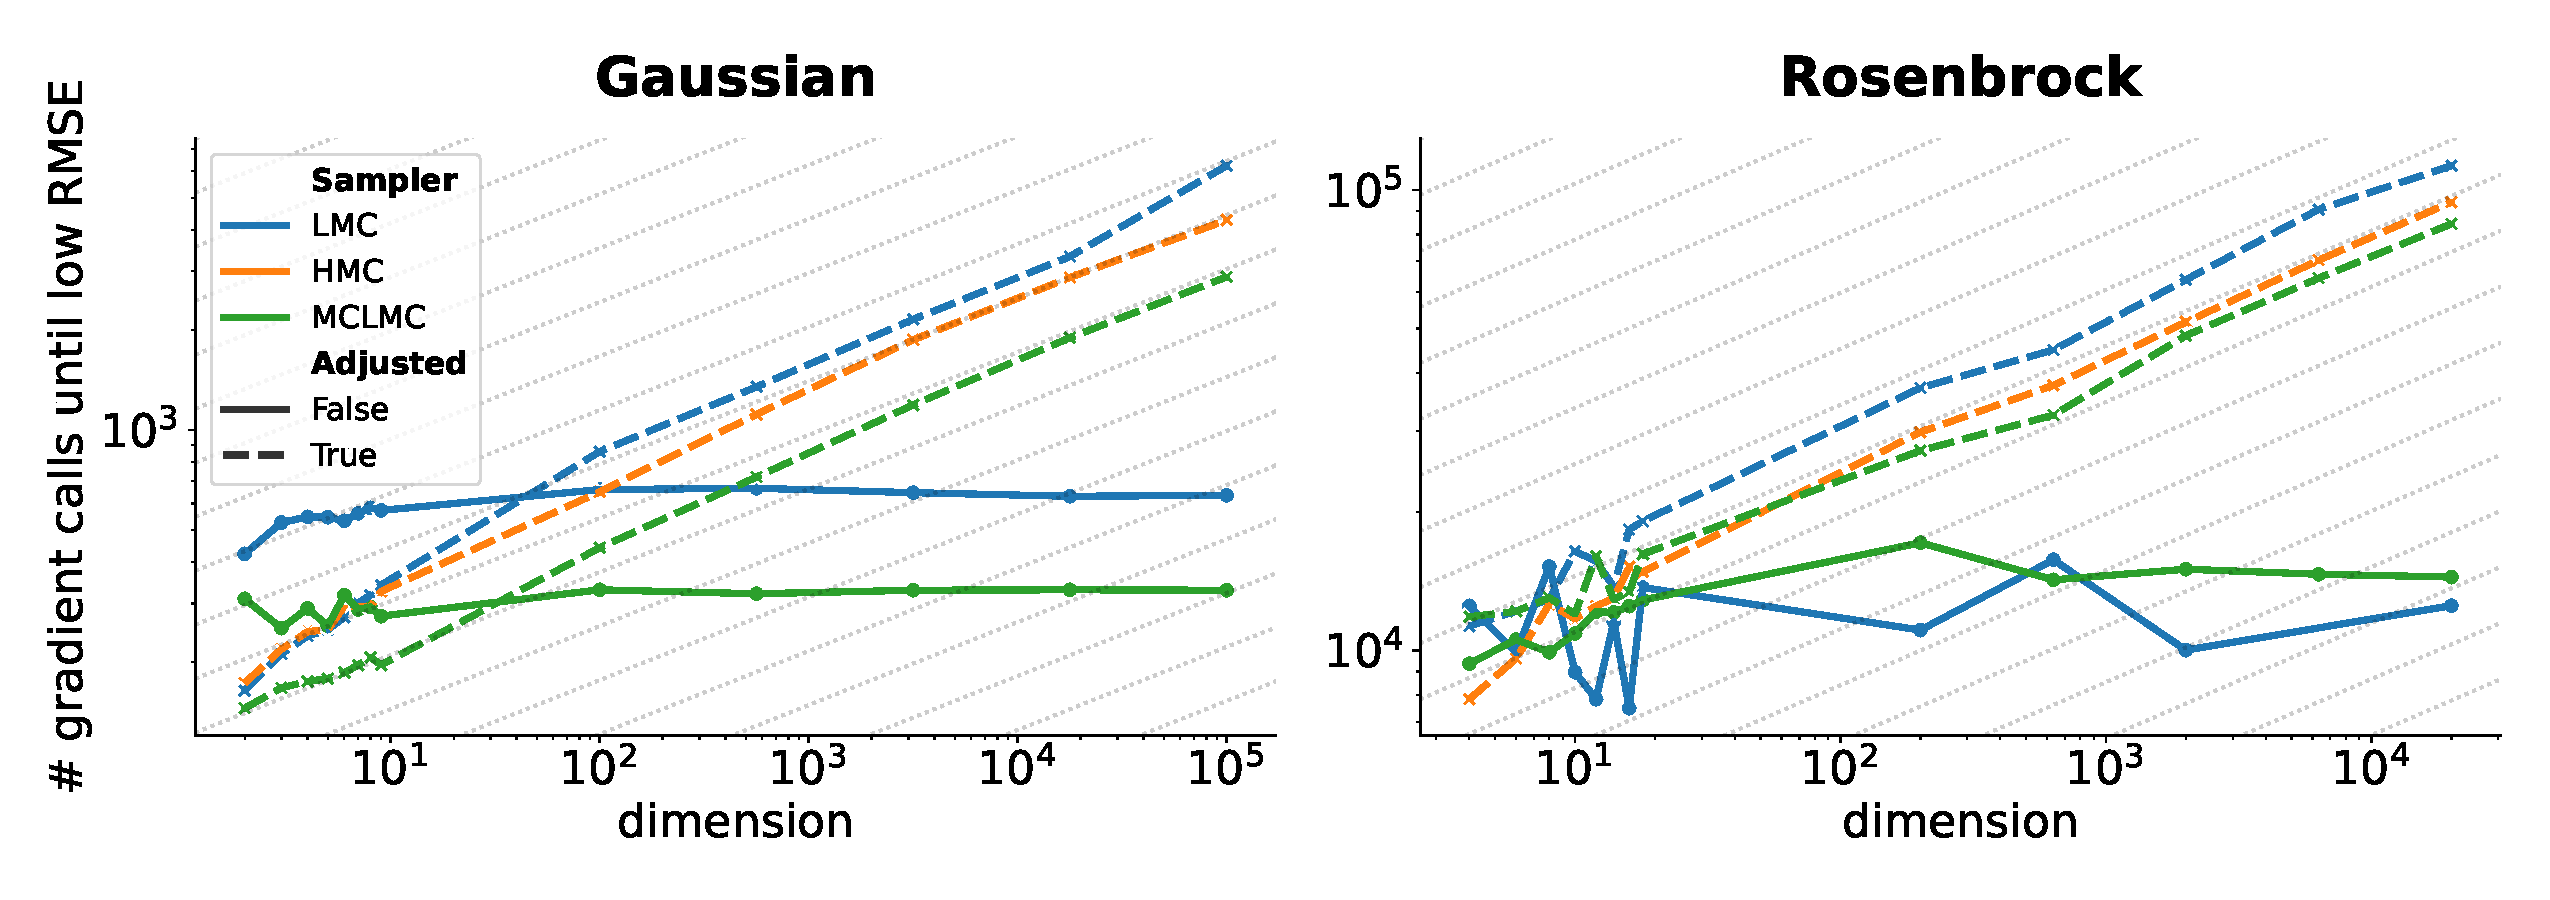
\includegraphics[width=0.95\linewidth]{figures/hmc/scaling.pdf}\\[0.2em]
      {\scriptsize Adjusted cost $\sim d^{1/4}$; unadjusted stays flat.}
    \end{column}
    \begin{column}{0.48\textwidth}
      \centering
      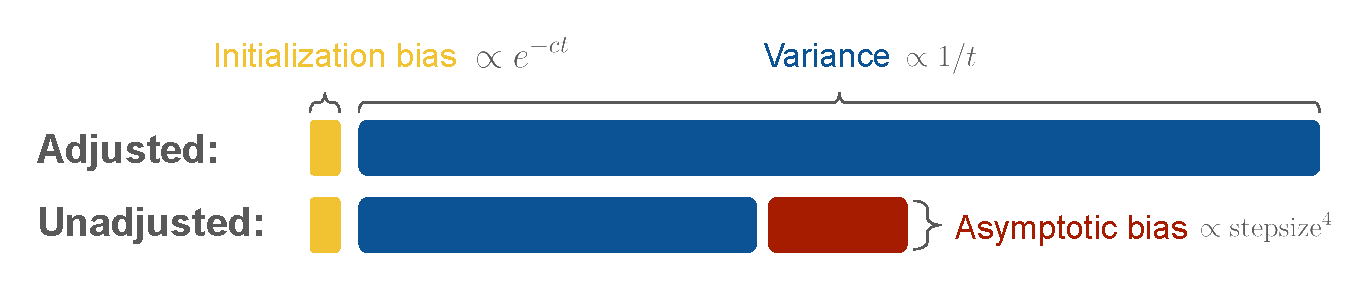
\includegraphics[width=0.95\linewidth]{figures/hmc/bias-variance-diagram.pdf}\\[0.2em]
      {\scriptsize Bias--variance: controlled bias, larger ESS.}
    \end{column}
  \end{columns}
\end{frame}

\begin{frame}{Back to physics: a spin--fermion model}
  Collaboration with \textbf{Peter Lunts} (formerly CCQ):
  unadjusted / microcanonical HMC for a lattice \textbf{spin--fermion} model.

  Two variance sources make this a good stress test:
  \begin{enumerate}\setlength\itemsep{0.35em}
    \item \textbf{Disorder} --- quenched randomness in AFM exchanges.
    \item \textbf{Hutchinson trace trick} --- stochastic traces for fermionic
      observables (noisy gradients / observables).
  \end{enumerate}
  \[
    S[\psi,\bar\psi,n]
    =
    S_{\mathrm{F}}[\psi,\bar\psi]
    +
    S_{\mathrm{b}}[n]
    +
    g\, n\cdot \bar\psi\,\sigma\,\psi
  \]
\end{frame}

\begin{frame}{Results: fermionic observables}
  From \emph{Fast Accurate Quantum Monte Carlo without Metropolis Adjustment}:
  \begin{center}
    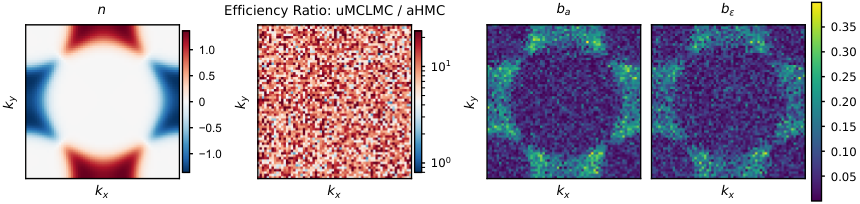
\includegraphics[width=0.95\linewidth]{figures/hmc/results/panel_longrun.png}
  \end{center}
  {\scriptsize $n(\mathbf{k})$; uMCLMC / aHMC efficiency; asymptotic bias $b_a$ and diagnostic $b_\epsilon$.}
\end{frame}

\begin{frame}{Results: efficiency vs~$\lambda$}
  \begin{columns}[T]
    \begin{column}{0.55\textwidth}
      \centering
      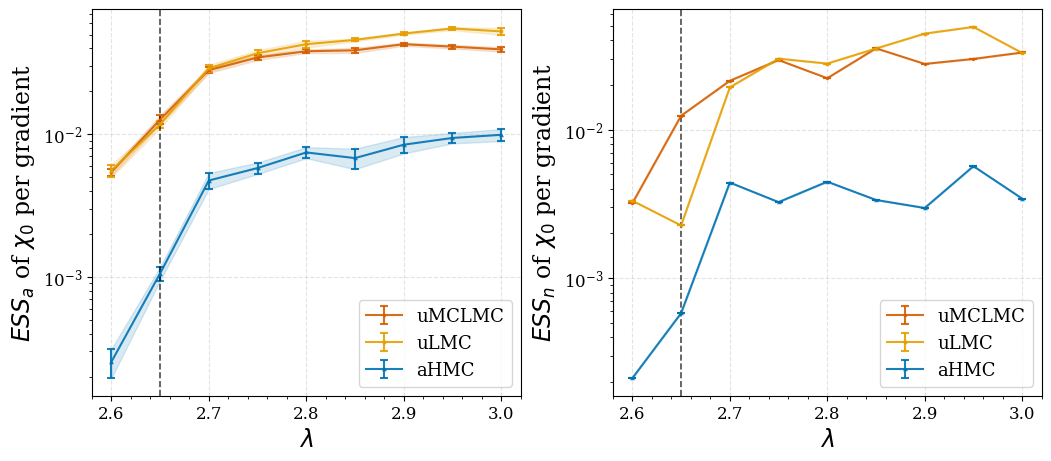
\includegraphics[width=\linewidth]{figures/hmc/results/efficiency_plot.png}
    \end{column}
    \begin{column}{0.42\textwidth}
      \begin{itemize}
        \item Unadjusted \textbf{uMCLMC} / \textbf{uLMC} beat adjusted HMC by roughly an order of magnitude in ESS per gradient
        \item Accuracy matched (bias controlled by step-size tuning)
        \item Gains grow with system size
      \end{itemize}
    \end{column}
  \end{columns}
\end{frame}

\section{Functional reactive programming}
\renewcommand{\currentEdge}{stats-fp}

\begin{frame}{Statistics + Functional Programming}
  \begin{center}
    \ResearchTriangle{stats-fp}
  \end{center}
\end{frame}

\begin{frame}{The na\"ive workflow}
  A natural way to do statistical programming:
  \begin{enumerate}\setlength\itemsep{0.4em}
    \item Derive the model on a whiteboard
      (the Markov kernels you want: prior, likelihood, filter,\ldots)
    \item Hand-write a program that implements those kernels
  \end{enumerate}
  \vspace{0.6em}
  Laborious --- and risky:
  \begin{itemize}\setlength\itemsep{0.3em}
    \item No guarantee of a \textbf{link} between the mathematical model
      and the running program
    \item Every change to the model reopens the derivation
  \end{itemize}
\end{frame}

\begin{frame}{Probabilistic programming}
  \textbf{Idea:} specify the \emph{model} as code;\\
  automate the derivation of the inference method.
  \vspace{0.8em}
  \begin{columns}[c]
    \begin{column}{0.48\textwidth}
      \centering
      {\large whiteboard $\;\to\;$ program}\\[0.4em]
      {\small hand-derived kernels}
    \end{column}
    \begin{column}{0.04\textwidth}
      \centering$\Longrightarrow$
    \end{column}
    \begin{column}{0.48\textwidth}
      \centering
      {\large model-as-code $\;\to\;$ inference}\\[0.4em]
      {\small compiler / library derives the sampler}
    \end{column}
  \end{columns}
  \vspace{1em}
  \textbf{Stan} is the canonical example:\\
  write a generative model; get HMC for free.
\end{frame}

\begin{frame}[fragile]{Warm-up: static particle detection}
  A particle at unknown position $x$; one noisy observation $y$.
  \vspace{0.4em}
  \begin{columns}[T]
    \begin{column}{0.55\textwidth}
\begin{semiverbatim}
-- monad-bayes style
detect :: MonadInfer m => Double -> m Double
detect y = do
  x <- normal 0 1           -- prior
  score (normalPdf x 0.5 y) -- likelihood
  return x                  -- posterior sample
\end{semiverbatim}
    \end{column}
    \begin{column}{0.45\textwidth}
      \[
        \begin{aligned}
          x &\sim \mathcal{N}(0,1) \\
          y \mid x &\sim \mathcal{N}(x, 0.5^2)
        \end{aligned}
      \]
      \vspace{0.3em}
      {\small Model = generative story + conditioning.}
    \end{column}
  \end{columns}
\end{frame}

\begin{frame}{Many inference methods}
  Same model; many ways to draw from $p(x\mid y)$:
  \begin{columns}[T]
    \begin{column}{0.5\textwidth}
      \begin{itemize}\setlength\itemsep{0.25em}
        \item Exact conjugate update
        \item Importance sampling / SMC
        \item Metropolis--Hastings
        \item \textbf{HMC} (Stan's default)
        \item Variational inference
      \end{itemize}
    \end{column}
    \begin{column}{0.5\textwidth}
      The PPL's job: \textbf{choose / derive} an
      inference method from the model code.

      \vspace{0.6em}
      {\small Stan $\approx$ HMC for static models.}

      \vspace{0.4em}
      {\small What about models that unfold in \textbf{time}?}
    \end{column}
  \end{columns}
\end{frame}

\begin{frame}{A PPL for stochastic processes}
  Stan targets \textbf{static} models (batch data, fixed dimension).

  \vspace{0.5em}
  I've been building a probabilistic programming language for
  \textbf{stochastic processes}: models that unfold in time,
  with streaming observations and online inference.

  \vspace{0.6em}
  Built in Haskell by fusing
  \begin{itemize}\setlength\itemsep{0.25em}
    \item \textbf{functional reactive programming} --- signal functions over time
    \item \textbf{probabilistic programming} --- sampling, conditioning, SMC
  \end{itemize}
\end{frame}

% --- Live demo: ball with noisy observations ---------------------------------
% Preferred: Quarto/Reveal deck embeds WASM demo1 and stages via
% .frp-demo-slot[data-frp-stage=prior|obs|hidden|particles].
% Beamer: run the browser demo alongside, or advance these frames as cues.

\begin{frame}[fragile]{Demo: prior dynamics}
  \begin{columns}[T]
    \begin{column}{0.46\textwidth}
      \textbf{Live:} latent ball only\\[0.3em]
      {\small (teal = true position)}
      \vspace{1.2em}

      {\scriptsize\textit{[Reveal: live WASM embed]}}
    \end{column}
    \begin{column}{0.54\textwidth}
\begin{semiverbatim}
prior :: () >--> Position
prior = proc _ -> do
  x <- stochasticOscillator 0 0 -< 1
  y <- stochasticOscillator 0 0 -< 1
  returnA -< V2 x y
\end{semiverbatim}
      \vspace{0.4em}
      {\small A noisy harmonic oscillator --- a stochastic process.}
    \end{column}
  \end{columns}
\end{frame}

\begin{frame}[fragile]{Demo: observation model}
  \begin{columns}[T]
    \begin{column}{0.46\textwidth}
      \textbf{Live:} latent + noisy observations\\[0.3em]
      {\small (red = what the system sees)}
      \vspace{1.2em}

      {\scriptsize\textit{[demo: + observations]}}
    \end{column}
    \begin{column}{0.54\textwidth}
\begin{semiverbatim}
observationModel ::
  Position >--> Observation
observationModel = proc p -> do
  nx <- noise -< ()
  ny <- noise -< ()
  returnA -< p + V2 nx ny
  where
    noise = constM (normal 0 std)
\end{semiverbatim}
    \end{column}
  \end{columns}
\end{frame}

\begin{frame}[fragile]{Demo: the inference problem}
  \begin{columns}[T]
    \begin{column}{0.46\textwidth}
      \textbf{Live:} hide / shade the latent\\[0.3em]
      {\small Only observations remain visible.}
      \vspace{1.2em}

      {\scriptsize\textit{[demo: latent off]}}
      \vspace{0.8em}

      {\small Infer $p(\mathrm{position}_t \mid \mathrm{obs}_{\le t})$.}
    \end{column}
    \begin{column}{0.54\textwidth}
\begin{semiverbatim}
posterior ::
  Observation >-/-> Position
posterior = proc obs -> do
  latent <- prior -< ()
  observe -<
    likelihood obs latent
  returnA -< latent
\end{semiverbatim}
      \vspace{0.4em}
      {\small Unnormalized: model + conditioning, not yet a sampler.}
    \end{column}
  \end{columns}
\end{frame}

\begin{frame}[fragile]{Demo: automated inference}
  \begin{columns}[T]
    \begin{column}{0.46\textwidth}
      \textbf{Live:} particle cloud\\[0.3em]
      {\small (purple = posterior particles)}
      \vspace{1.2em}

      {\scriptsize\textit{[demo: + particles]}}
    \end{column}
    \begin{column}{0.54\textwidth}
\begin{semiverbatim}
inference :: Observation
          >--> [(Position, Weight)]
inference =
  particleFilter params \{n = 100\}
    posterior
\end{semiverbatim}
      \vspace{0.6em}
      {\small Same model code; SMC is derived by the library ---\\
      analogous to Stan automating HMC.}
    \end{column}
  \end{columns}
\end{frame}

\section{Typed fusion}
\renewcommand{\currentEdge}{fp-physics}

\begin{frame}{Functional Programming + Physics}
  \begin{center}
    \ResearchTriangle{fp-physics}
  \end{center}
\end{frame}

\begin{frame}{Little contact so far}
  Functional programming and programming-language theory
  have made \textbf{little contact} with computational physics.

  \vspace{0.8em}
  \begin{columns}[T]
    \begin{column}{0.48\textwidth}
      \textbf{Understandable}
      \begin{itemize}\setlength\itemsep{0.35em}
        \item Performance is the priority
        \item You want hardware control
        \item Imperative / low-level tools dominate
      \end{itemize}
    \end{column}
    \begin{column}{0.48\textwidth}
      \textbf{But appealing}
      \begin{itemize}\setlength\itemsep{0.35em}
        \item Specs of algorithms can be very rich
        \item Lots of structure to encode
        \item Types / abstraction can pull their weight
      \end{itemize}
    \end{column}
  \end{columns}
\end{frame}

\begin{frame}{A mathematically rich domain}
  \textbf{Example:} group representations
  (e.g.\ $SU(2)$ spins in quantum many-body physics).

  \vspace{0.7em}
  Symmetry-respecting maps (intertwiners) carry nontrivial structure:
  \begin{itemize}\setlength\itemsep{0.35em}
    \item Tensor products fuse: $\tfrac12\otimes\tfrac12 \;\cong\; 1\oplus 0$
    \item Data lives in \textbf{blocks} indexed by irreps
    \item Shapes are dictated by representation theory --- not by ad hoc bookkeeping
  \end{itemize}

  \vspace{0.6em}
  {\small Natural question: can the type system track this structure?}
\end{frame}

\begin{frame}[fragile]{Length-checked linear algebra}
  Start simple: dimensions in the types.
  \vspace{0.5em}
\begin{semiverbatim}
vectorExample :: C 3
vectorExample = vec (1,2,3)

tensorProductExample :: C 3 ⊗ C 2
tensorProductExample =
  vec (1,2,3) ⊗ vec (4,5)
\end{semiverbatim}
  \vspace{0.5em}
  Wrong length $\Rightarrow$ \textbf{compile-time} error --- not a silent
  reshape bug at runtime.
\end{frame}

\begin{frame}[fragile]{Irreps as types}
  Same idea, but the ``length'' is a representation:
  \vspace{0.5em}
\begin{semiverbatim}
irrepExample ::
  VectorOf SU2 (Irrep (Spin (1/2)))
irrepExample = vec (1,2)

directSumOfIrrepsExample ::
  Unfused SU2
    (Irrep (Spin (1/2))
       :⊕: Irrep (Spin (3/2)))
directSumOfIrrepsExample =
  (vec (1,2), vec (3,4,5,6))
\end{semiverbatim}
  \vspace{0.4em}
  {\small $\mathbb{C}^2$ for spin-$\tfrac12$; $\mathbb{C}^4$ for spin-$\tfrac32$ --- checked by the type.}
\end{frame}

\begin{frame}[fragile]{Fusion at the type level}
  Tensor products of irreps \textbf{fuse}:
  $\tfrac12\otimes\tfrac12 \;\cong\; 0\oplus 1$.
  \vspace{0.45em}
\begin{semiverbatim}
unfused :: Unfused SU2
  (Irrep (Spin (1/2)) :⊗: Irrep (Spin (1/2)))
unfused = mat ((1,2),(5,6))   -- ℂ² ⊗ ℂ²

fused :: Fused SU2
  (Irrep (Spin (1/2)) :⊗: Irrep (Spin (1/2)))
fused = (konst 1, vec (4,5,6))  -- ℂ¹ ⊕ ℂ³
\end{semiverbatim}
  \vspace{0.45em}
  Haskell computes the fused shape \textbf{at compile time};\\
  a wrong block size is rejected before you run anything.
\end{frame}

\begin{frame}[fragile]{Keeping only the trivial sector}
  Intertwiners live in the invariant ($j{=}0$) subspace ---
  Schur's lemma as a type:
  \vspace{0.45em}
\begin{semiverbatim}
trivialSectorExample ::
  Sym SU2
    (Irrep (Spin (1/2)) :⊗: Irrep (Spin (1/2)))
trivialSectorExample = konst 2   -- ℂ¹

-- 3/2 ⊗ 1/2 = 1 ⊕ 2  (no singlet)
trivialSectorExample2 ::
  Sym SU2
    (Irrep (Spin (3/2)) :⊗: Irrep (Spin (1/2)))
trivialSectorExample2 = EmptyFTrees
\end{semiverbatim}
\end{frame}

\begin{frame}[fragile]{From fusion to categories}
  Once objects are typed, morphisms compose by the
  \textbf{same} abstract law in every fusion category.
  \vspace{0.4em}
\begin{semiverbatim}
-- Mac Lane ladder on names ⌜f⌝, ⌜g⌝:
composeNames @Fib  nf ng
composeNames @Ising nf ng
\end{semiverbatim}
  \vspace{0.5em}
  \[
    \lceil f\rceil\otimes\lceil g\rceil
    \;\xrightarrow{\;\alpha,\;\varepsilon,\;\lambda\;}\;
    \lceil g\circ f\rceil
  \]
  \vspace{0.3em}
  Fibonacci and Ising share one implementation ---\\
  the mathematics supplies the abstraction boundary.
\end{frame}

\begin{frame}{Design principle}
  The mathematics shows how to \textbf{abstract} and
  \textbf{design} the software:
  \begin{itemize}\setlength\itemsep{0.45em}
    \item Representation theory $\;\Rightarrow\;$ block shapes in the types
    \item Fusion rules $\;\Rightarrow\;$ checked at compile time
    \item Compact closed structure $\;\Rightarrow\;$ one compositional API
      across theories (SU(2), Fib, Ising, \ldots)
  \end{itemize}

  \vspace{0.7em}
  {\small Code that looks like the maths --- not an imperative simulation
  with the same numeric answers.}
\end{frame}

\section{Outlook}
\renewcommand{\currentEdge}{all}

\begin{frame}{Outlook}
  % TODO: synthesis across the three strands
\end{frame}

\begin{frame}{Fit with CCQ}
  % TODO: collaborations, software culture, future directions
\end{frame}


\end{document}
